\documentclass{standalone}
\usepackage{tikz}
\usetikzlibrary{patterns, positioning}


\begin{document}
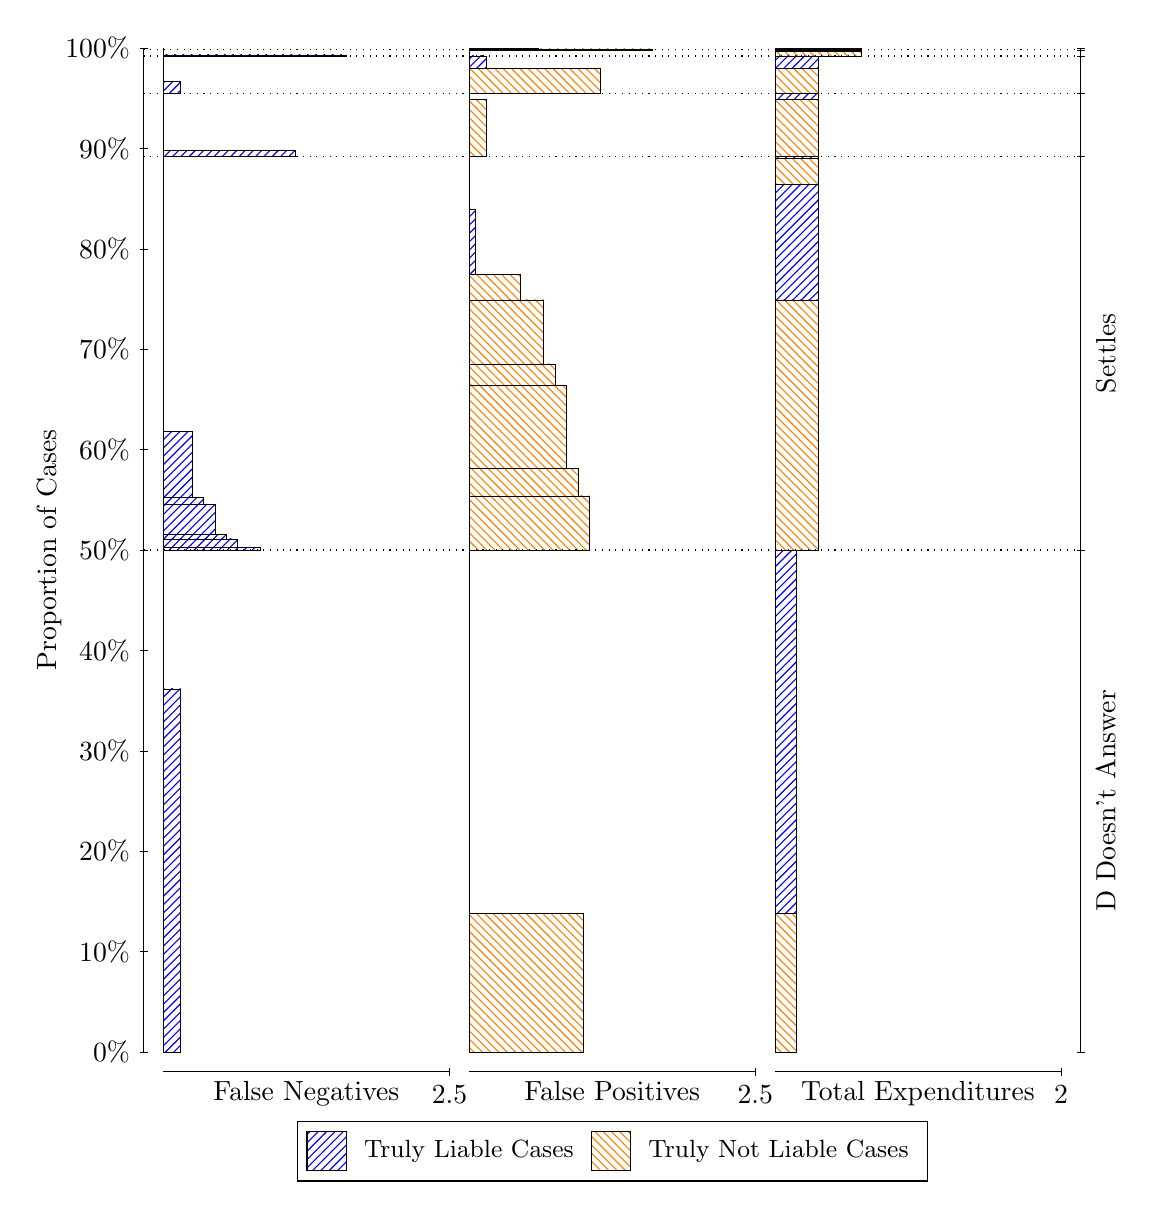
\begin{tikzpicture}
\draw[black, very thin] (1.5,1.75) -- (1.5,14.5);
\node[rotate=90, text=black, anchor=center] at (0.3, 8.125) {Proportion of Cases};
\draw[black, very thin] (1.45,1.75) -- (1.55,1.75);
\node[text=black, anchor=east] at (1.45, 1.75) {0\%};
\draw[black, very thin] (1.45,3.025) -- (1.55,3.025);
\node[text=black, anchor=east] at (1.45, 3.025) {10\%};
\draw[black, very thin] (1.45,4.3) -- (1.55,4.3);
\node[text=black, anchor=east] at (1.45, 4.3) {20\%};
\draw[black, very thin] (1.45,5.575) -- (1.55,5.575);
\node[text=black, anchor=east] at (1.45, 5.575) {30\%};
\draw[black, very thin] (1.45,6.85) -- (1.55,6.85);
\node[text=black, anchor=east] at (1.45, 6.85) {40\%};
\draw[black, very thin] (1.45,8.125) -- (1.55,8.125);
\node[text=black, anchor=east] at (1.45, 8.125) {50\%};
\draw[black, very thin] (1.45,9.4) -- (1.55,9.4);
\node[text=black, anchor=east] at (1.45, 9.4) {60\%};
\draw[black, very thin] (1.45,10.675) -- (1.55,10.675);
\node[text=black, anchor=east] at (1.45, 10.675) {70\%};
\draw[black, very thin] (1.45,11.95) -- (1.55,11.95);
\node[text=black, anchor=east] at (1.45, 11.95) {80\%};
\draw[black, very thin] (1.45,13.225) -- (1.55,13.225);
\node[text=black, anchor=east] at (1.45, 13.225) {90\%};
\draw[black, very thin] (1.45,14.5) -- (1.55,14.5);
\node[text=black, anchor=east] at (1.45, 14.5) {100\%};

\draw[black, very thin] (13.4,1.75) -- (13.4,14.5);
\draw[black, very thin] (13.35,1.75) -- (13.45,1.75);
\node[anchor=west] at (13.35, 1.75) {};
\draw[black, very thin] (13.35,8.1249) -- (13.45,8.1249);
\node[anchor=west] at (13.35, 8.1249) {};
\draw[black, very thin] (13.35,13.124) -- (13.45,13.124);
\node[anchor=west] at (13.35, 13.124) {};
\draw[black, very thin] (13.35,13.92) -- (13.45,13.92);
\node[anchor=west] at (13.35, 13.92) {};
\draw[black, very thin] (13.35,14.399) -- (13.45,14.399);
\node[anchor=west] at (13.35, 14.399) {};
\draw[black, very thin] (13.35,14.476) -- (13.45,14.476);
\node[anchor=west] at (13.35, 14.476) {};
\draw[black, very thin] (13.35,14.5) -- (13.45,14.5);
\node[anchor=west] at (13.35, 14.5) {};

\draw[black, very thin, pattern color=blue, pattern=north east lines] (1.75,1.75) rectangle (1.968,6.3601);
\draw[black, very thin, pattern color=orange, pattern=north west lines] (1.75,6.3601) rectangle (1.75,8.1249);
\draw[black, very thin, pattern color=blue, pattern=north east lines] (1.75,8.1249) rectangle (2.9853,8.1556);
\draw[black, very thin, pattern color=blue, pattern=north east lines] (1.75,8.1556) rectangle (2.6947,8.2661);
\draw[black, very thin, pattern color=blue, pattern=north east lines] (1.75,8.2661) rectangle (2.5493,8.3261);
\draw[black, very thin, pattern color=blue, pattern=north east lines] (1.75,8.3261) rectangle (2.404,8.6996);
\draw[black, very thin, pattern color=blue, pattern=north east lines] (1.75,8.6996) rectangle (2.2587,8.793);
\draw[black, very thin, pattern color=blue, pattern=north east lines] (1.75,8.793) rectangle (2.1133,9.6274);
\draw[black, very thin, pattern color=orange, pattern=north west lines] (1.75,9.6274) rectangle (1.75,13.124);
\draw[black, very thin, pattern color=blue, pattern=north east lines] (1.75,13.124) rectangle (3.4213,13.202);
\draw[black, very thin, pattern color=orange, pattern=north west lines] (1.75,13.202) rectangle (1.75,13.92);
\draw[black, very thin, pattern color=blue, pattern=north east lines] (1.75,13.92) rectangle (1.968,14.081);
\draw[black, very thin, pattern color=orange, pattern=north west lines] (1.75,14.081) rectangle (1.75,14.399);
\draw[black, very thin, pattern color=blue, pattern=north east lines] (1.75,14.399) rectangle (4.0753,14.412);
\draw[black, very thin, pattern color=orange, pattern=north west lines] (1.75,14.412) rectangle (1.75,14.476);
\draw[black, very thin, pattern color=orange, pattern=north west lines] (1.75,14.476) rectangle (1.75,14.489);
\draw[black, very thin, pattern color=blue, pattern=north east lines] (1.75,14.489) rectangle (1.75,14.5);
\draw[black, very thin, pattern color=orange, pattern=north west lines] (5.6333,1.75) rectangle (7.0867,3.5148);
\draw[black, very thin, pattern color=blue, pattern=north east lines] (5.6333,3.5148) rectangle (5.6333,8.1249);
\draw[black, very thin, pattern color=orange, pattern=north west lines] (5.6333,8.1249) rectangle (7.1593,8.8123);
\draw[black, very thin, pattern color=orange, pattern=north west lines] (5.6333,8.8123) rectangle (7.014,9.1575);
\draw[black, very thin, pattern color=orange, pattern=north west lines] (5.6333,9.1575) rectangle (6.8687,10.218);
\draw[black, very thin, pattern color=orange, pattern=north west lines] (5.6333,10.218) rectangle (6.7233,10.489);
\draw[black, very thin, pattern color=orange, pattern=north west lines] (5.6333,10.489) rectangle (6.578,11.3);
\draw[black, very thin, pattern color=orange, pattern=north west lines] (5.6333,11.3) rectangle (6.2873,11.622);
\draw[black, very thin, pattern color=blue, pattern=north east lines] (5.6333,11.622) rectangle (5.706,12.456);
\draw[black, very thin, pattern color=blue, pattern=north east lines] (5.6333,12.456) rectangle (5.6333,13.124);
\draw[black, very thin, pattern color=orange, pattern=north west lines] (5.6333,13.124) rectangle (5.8513,13.843);
\draw[black, very thin, pattern color=blue, pattern=north east lines] (5.6333,13.843) rectangle (5.6333,13.92);
\draw[black, very thin, pattern color=orange, pattern=north west lines] (5.6333,13.92) rectangle (7.3047,14.238);
\draw[black, very thin, pattern color=blue, pattern=north east lines] (5.6333,14.238) rectangle (5.8513,14.399);
\draw[black, very thin, pattern color=orange, pattern=north west lines] (5.6333,14.399) rectangle (5.6333,14.463);
\draw[black, very thin, pattern color=blue, pattern=north east lines] (5.6333,14.463) rectangle (5.6333,14.476);
\draw[black, very thin, pattern color=orange, pattern=north west lines] (5.6333,14.476) rectangle (7.9587,14.489);
\draw[black, very thin, pattern color=blue, pattern=north east lines] (5.6333,14.489) rectangle (6.5053,14.5);
\draw[black, very thin, pattern color=orange, pattern=north west lines] (9.5167,1.75) rectangle (9.7892,3.5148);
\draw[black, very thin, pattern color=blue, pattern=north east lines] (9.5167,3.5148) rectangle (9.7892,8.1249);
\draw[black, very thin, pattern color=orange, pattern=north west lines] (9.5167,8.1249) rectangle (10.062,11.3);
\draw[black, very thin, pattern color=blue, pattern=north east lines] (9.5167,11.3) rectangle (10.062,12.772);
\draw[black, very thin, pattern color=orange, pattern=north west lines] (9.5167,12.772) rectangle (10.062,13.094);
\draw[black, very thin, pattern color=blue, pattern=north east lines] (9.5167,13.094) rectangle (10.062,13.124);
\draw[black, very thin, pattern color=orange, pattern=north west lines] (9.5167,13.124) rectangle (10.062,13.843);
\draw[black, very thin, pattern color=blue, pattern=north east lines] (9.5167,13.843) rectangle (10.062,13.92);
\draw[black, very thin, pattern color=orange, pattern=north west lines] (9.5167,13.92) rectangle (10.062,14.238);
\draw[black, very thin, pattern color=blue, pattern=north east lines] (9.5167,14.238) rectangle (10.062,14.399);
\draw[black, very thin, pattern color=orange, pattern=north west lines] (9.5167,14.399) rectangle (10.607,14.463);
\draw[black, very thin, pattern color=blue, pattern=north east lines] (9.5167,14.463) rectangle (10.607,14.476);
\draw[black, very thin, pattern color=orange, pattern=north west lines] (9.5167,14.476) rectangle (10.607,14.489);
\draw[black, very thin, pattern color=blue, pattern=north east lines] (9.5167,14.489) rectangle (10.607,14.5);
\draw[black, dotted] (1.5,8.1249) -- (13.4,8.1249);
\draw[black, dotted] (1.5,13.124) -- (13.4,13.124);
\draw[black, dotted] (1.5,13.92) -- (13.4,13.92);
\draw[black, dotted] (1.5,14.399) -- (13.4,14.399);
\draw[black, dotted] (1.5,14.476) -- (13.4,14.476);
\draw[black, very thin] (1.75,1.5) -- (5.3833,1.5);
\node[text=black, anchor=north] at (3.5667, 1.5) {False Negatives};
\draw[black, very thin] (5.3833,1.45) -- (5.3833,1.55);
\node[text=black, anchor=north] at (5.3833, 1.45) {2.5};

\draw[black, very thin] (5.6333,1.5) -- (9.2667,1.5);
\node[text=black, anchor=north] at (7.45, 1.5) {False Positives};
\draw[black, very thin] (9.2667,1.45) -- (9.2667,1.55);
\node[text=black, anchor=north] at (9.2667, 1.45) {2.5};

\draw[black, very thin] (9.5167,1.5) -- (13.15,1.5);
\node[text=black, anchor=north] at (11.333, 1.5) {Total Expenditures};
\draw[black, very thin] (13.15,1.45) -- (13.15,1.55);
\node[text=black, anchor=north] at (13.15, 1.45) {2};

\node[text=black, centered, rotate=90] at (13.72, 4.9375) {D Doesn't Answer};
\node[text=black, centered, rotate=90] at (13.72, 10.625) {Settles};





\draw (7.449999999999999,1.5) node[draw=none] (baseCoordinate) {};
\begin{scope}[align=center]
        \matrix[scale=0.5, draw=black, below=0.5cm of baseCoordinate, nodes={draw}, column sep=0.1cm]{
            \node[rectangle, draw, minimum width=0.5cm, minimum height=0.5cm, pattern color=blue, pattern=north east lines] {}; &
            \node[draw=none, font=\small, text=black] (B) {Truly Liable Cases}; &
            \node[rectangle, draw, minimum width=0.5cm, minimum height=0.5cm, pattern color=orange, pattern=north west lines] {}; &
            \node[draw=none, font=\small, text=black] (B) {Truly Not Liable Cases}; \\
            };
\end{scope}

\end{tikzpicture}
\end{document}